% Content for Chapter 5, Section 5.5 — pulled in by chapters/05-system-design.tex
\subsection{مكوّنات الخدمة}

تضمّ هذه الخدمة ثماني عشرة خدمة تطبيقية، وهي أكبر خدمات النظام حجمًا. ويعرضها الشكل~\ref{fig:comp-02} مجمّعةً بحسب المسؤولية التي تملكها كل مجموعة.

\begin{figure}[htbp]
  \centering
  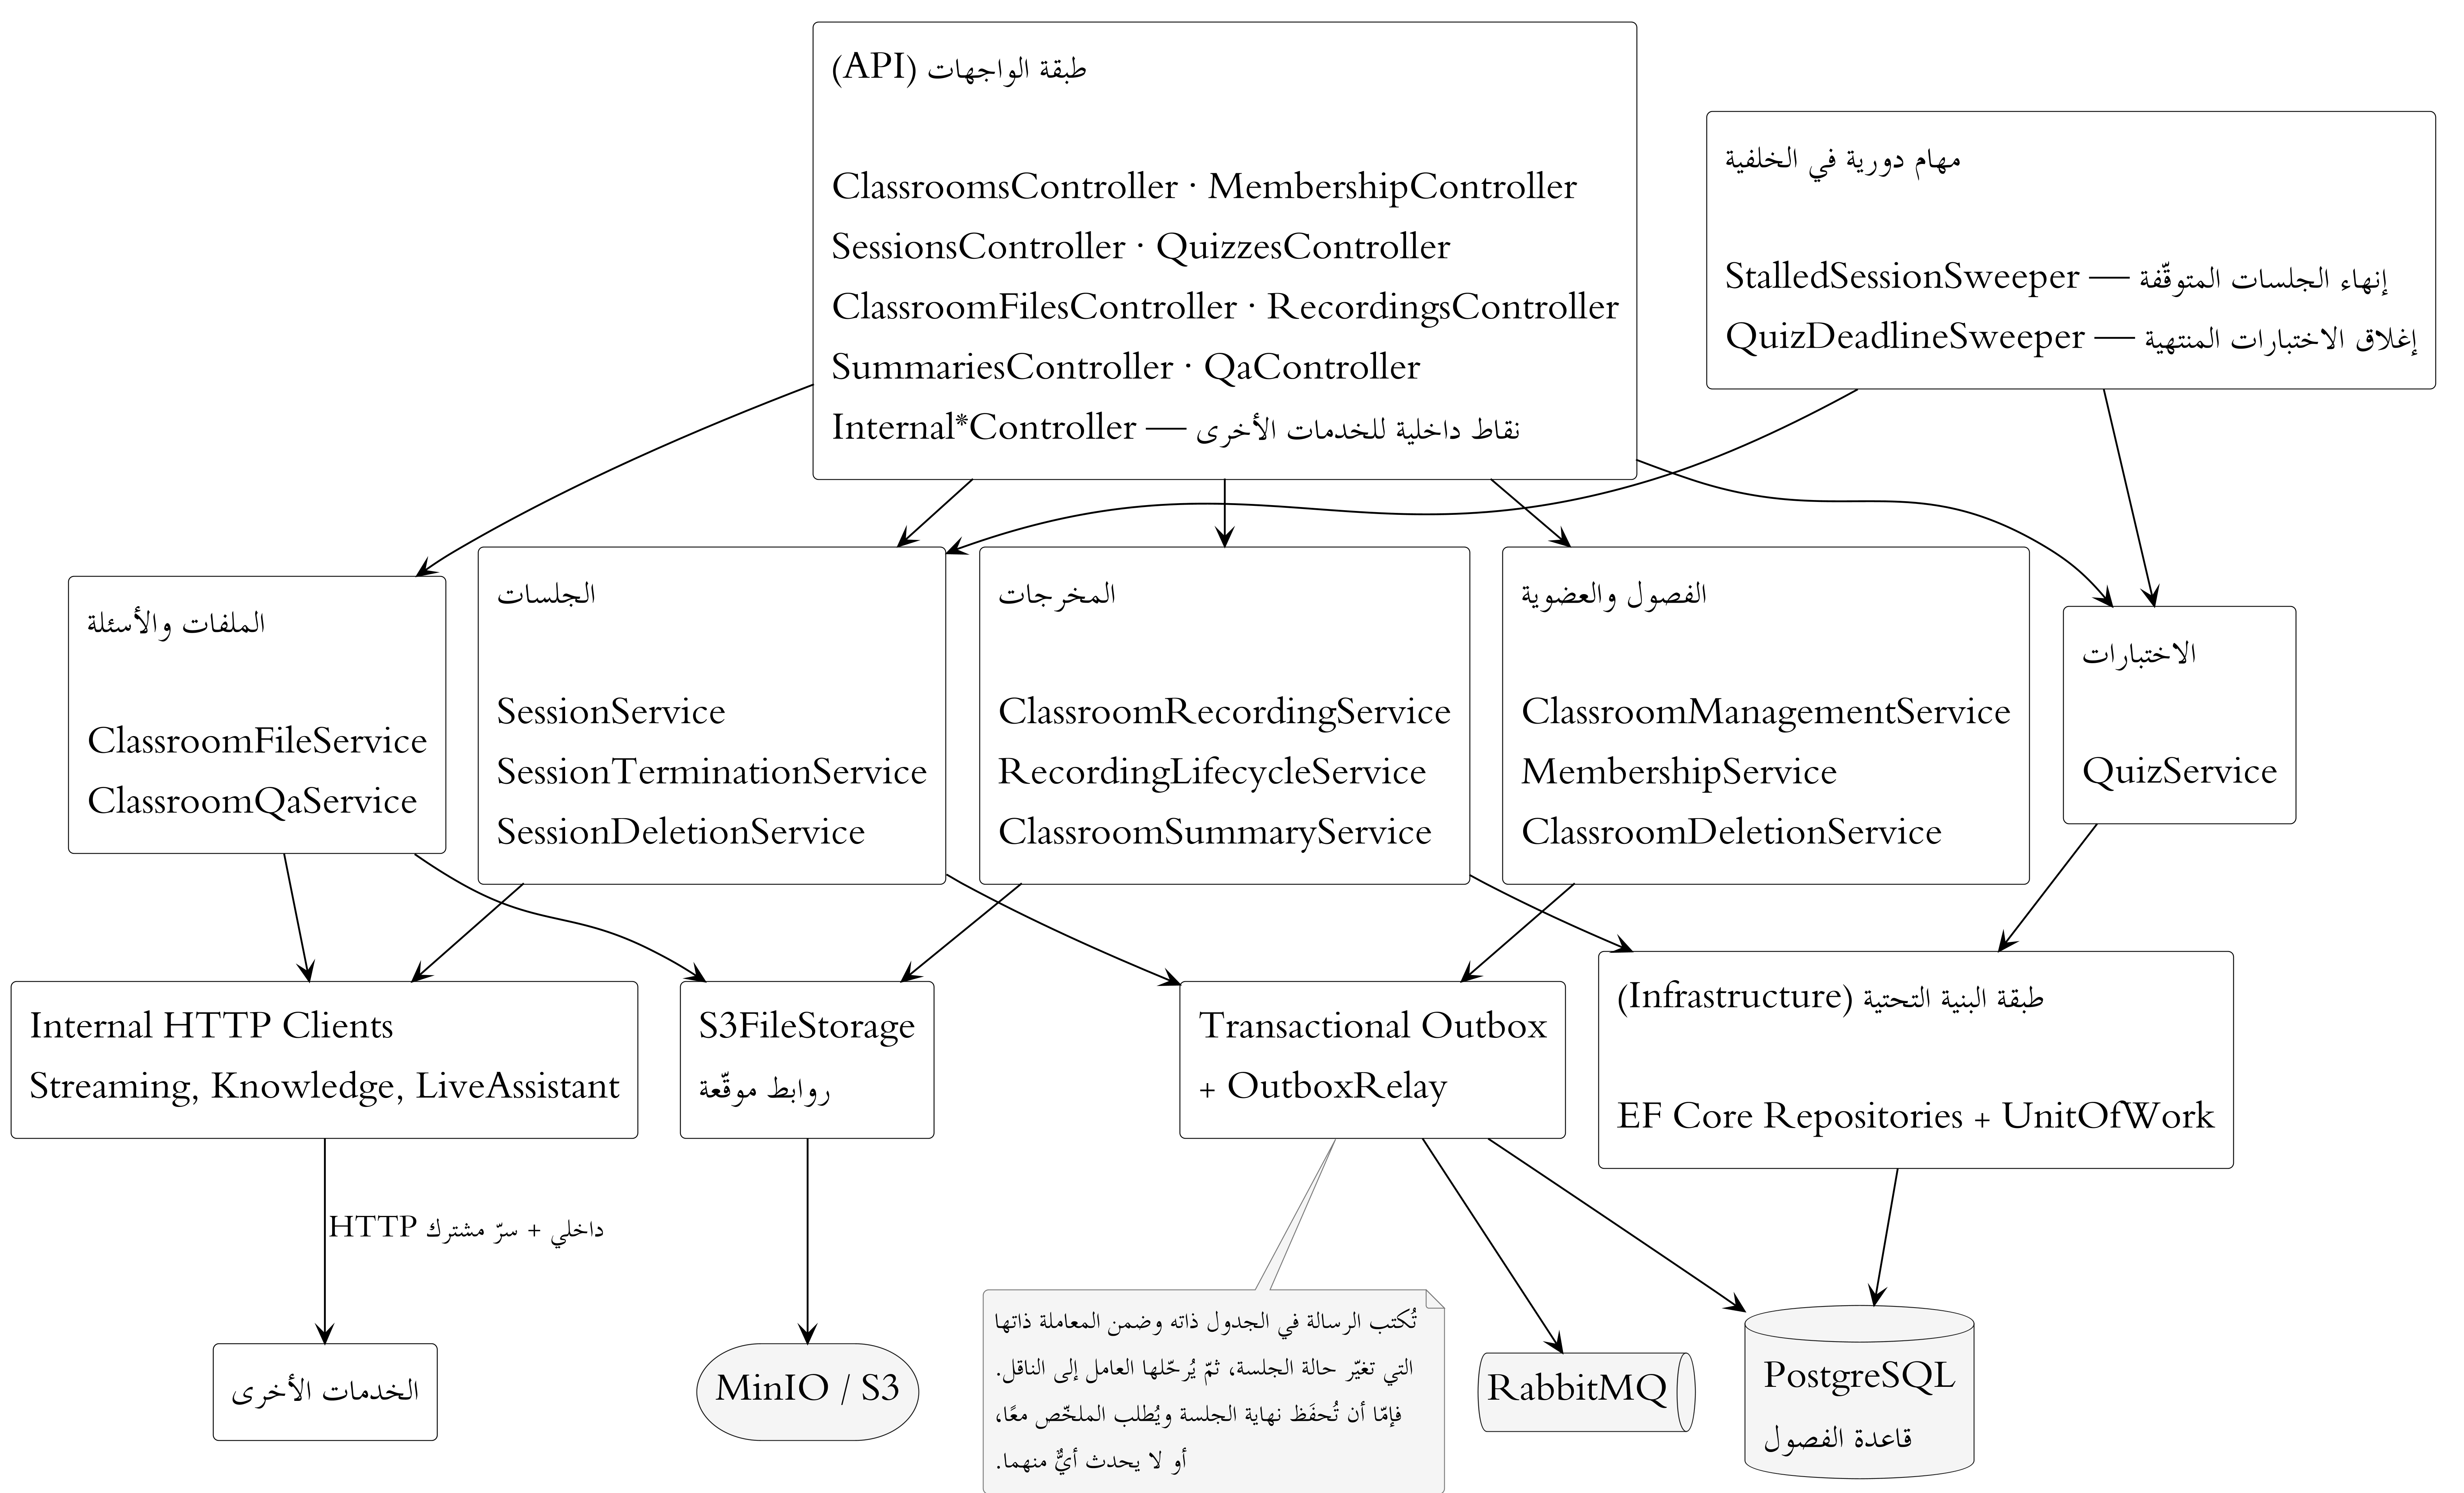
\includegraphics[width=\textwidth,height=0.8\textheight,keepaspectratio]{figures/comp-02-classroom.png}
  \caption{مخطط المكوّنات التفصيلي لخدمة الفصول الدراسية.}
  \label{fig:comp-02}
\end{figure}

وتظهر المهام الدورية في الخلفية منفصلةً عن بقية المكوّنات، لأنّها لا تُستدعى من أيّ مكوّن آخر بل تعمل على مؤقّتات. وتتولّى هذه المهام تصحيح الحالات الشاذّة، كانقطاع اتصال المعلّم في أثناء الجلسة أو انقضاء موعد إغلاق اختبار.

وترتبط هذه الخدمة بمحيطها عبر ثلاثة مسارات:

\begin{enumerate}
  \item \textbf{صندوق الصادر}: تنشر عبره أحداث المجال إلى الناقل.
  \item \textbf{مخزن الملفّات}: تحفظ فيه المواد المرجعية ومخرجات الجلسات، وتُصدر منه روابط موقَّعة محدودة المدّة.
  \item \textbf{عملاء \en{HTTP} الداخليون}: تُشغّل بهم الفهرسة في خدمة المعرفة، وتفكيك الغرف في خدمة البث، وتوليد الاختبارات في خدمة المساعد الحيّ.
\end{enumerate}

\subsection{نموذج البيانات}

يضمّ نموذج بيانات الخدمة اثني عشر كيانًا يعرضها الشكل~\ref{fig:erd-02}، موزّعةً على أربع مجموعات: الفصول وملفّاتها وعضويّاتها، والجلسات، ومخرجات الجلسات من تسجيلات وملخّصات، والاختبارات وهي المجموعة الأكبر.

\begin{figure}[htbp]
  \centering
  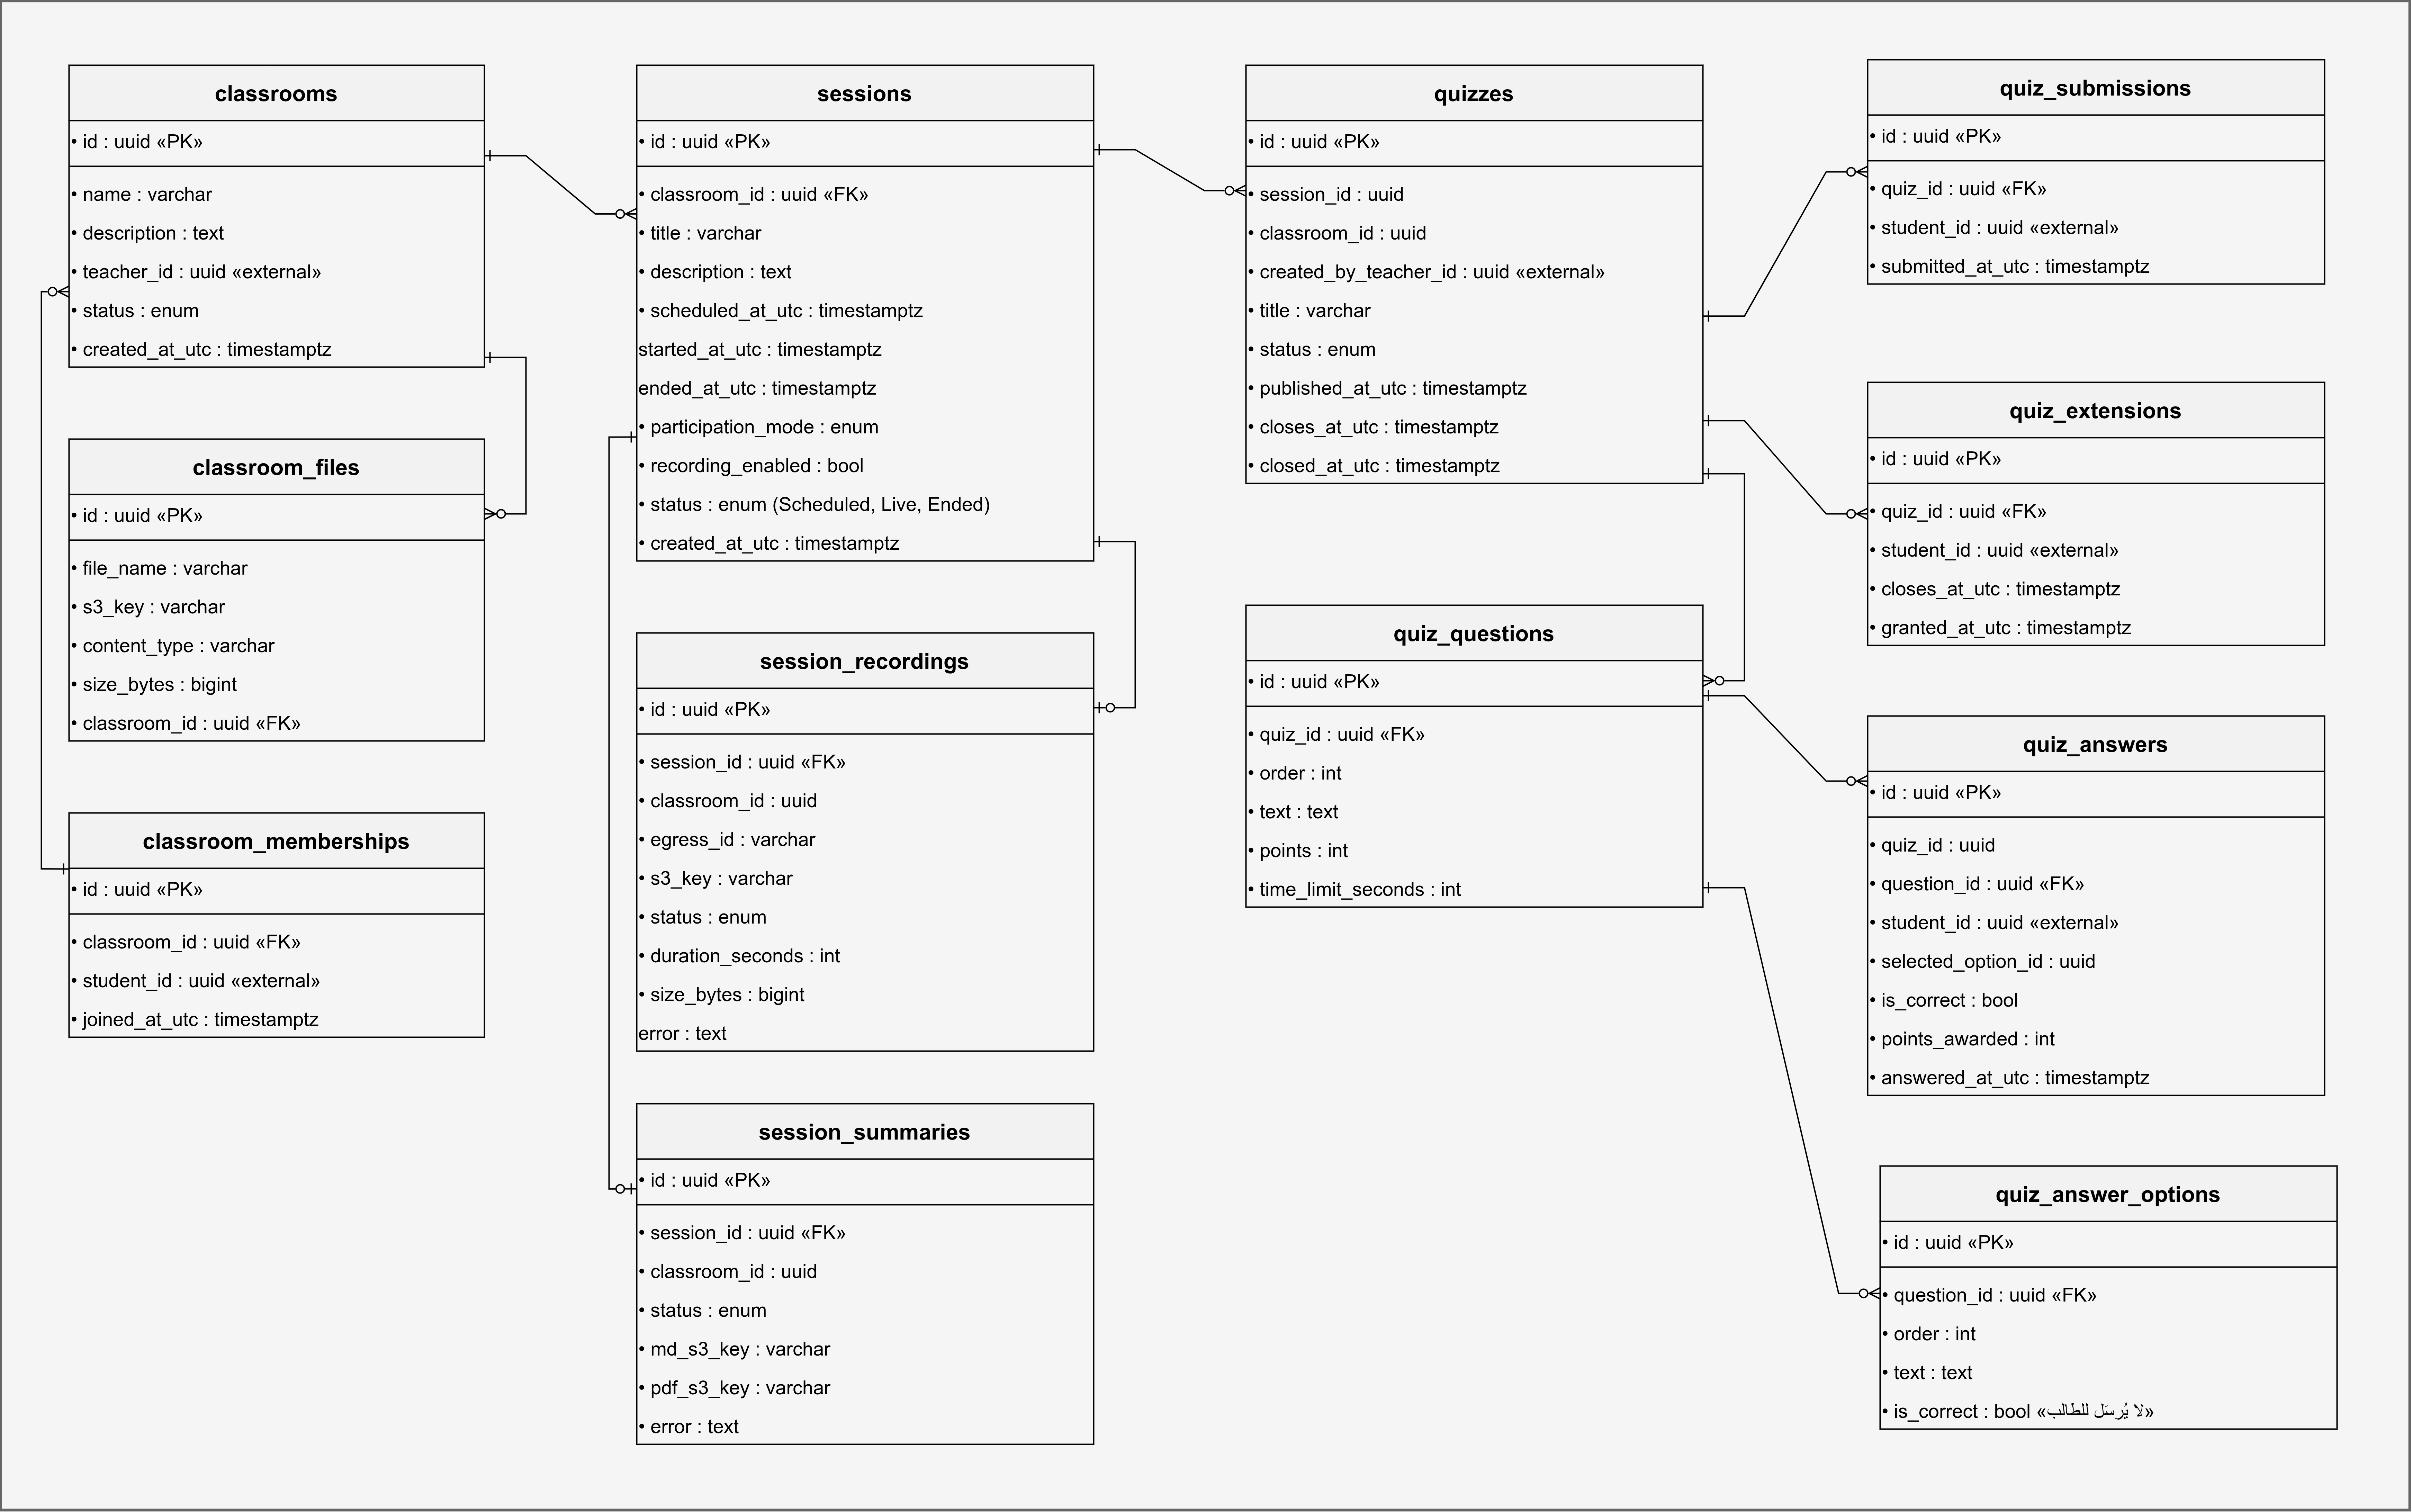
\includegraphics[width=\textwidth,height=0.8\textheight,keepaspectratio]{figures/erd-02-classroom.png}
  \caption{مخطط الكيانات والعلاقات لخدمة الفصول الدراسية.}
  \label{fig:erd-02}
\end{figure}

ويعرض الشكل~\ref{fig:class-02} تصميم تجميعة الاختبار (\en{Quiz Aggregate}) بمزيد من التفصيل.

\begin{figure}[htbp]
  \centering
  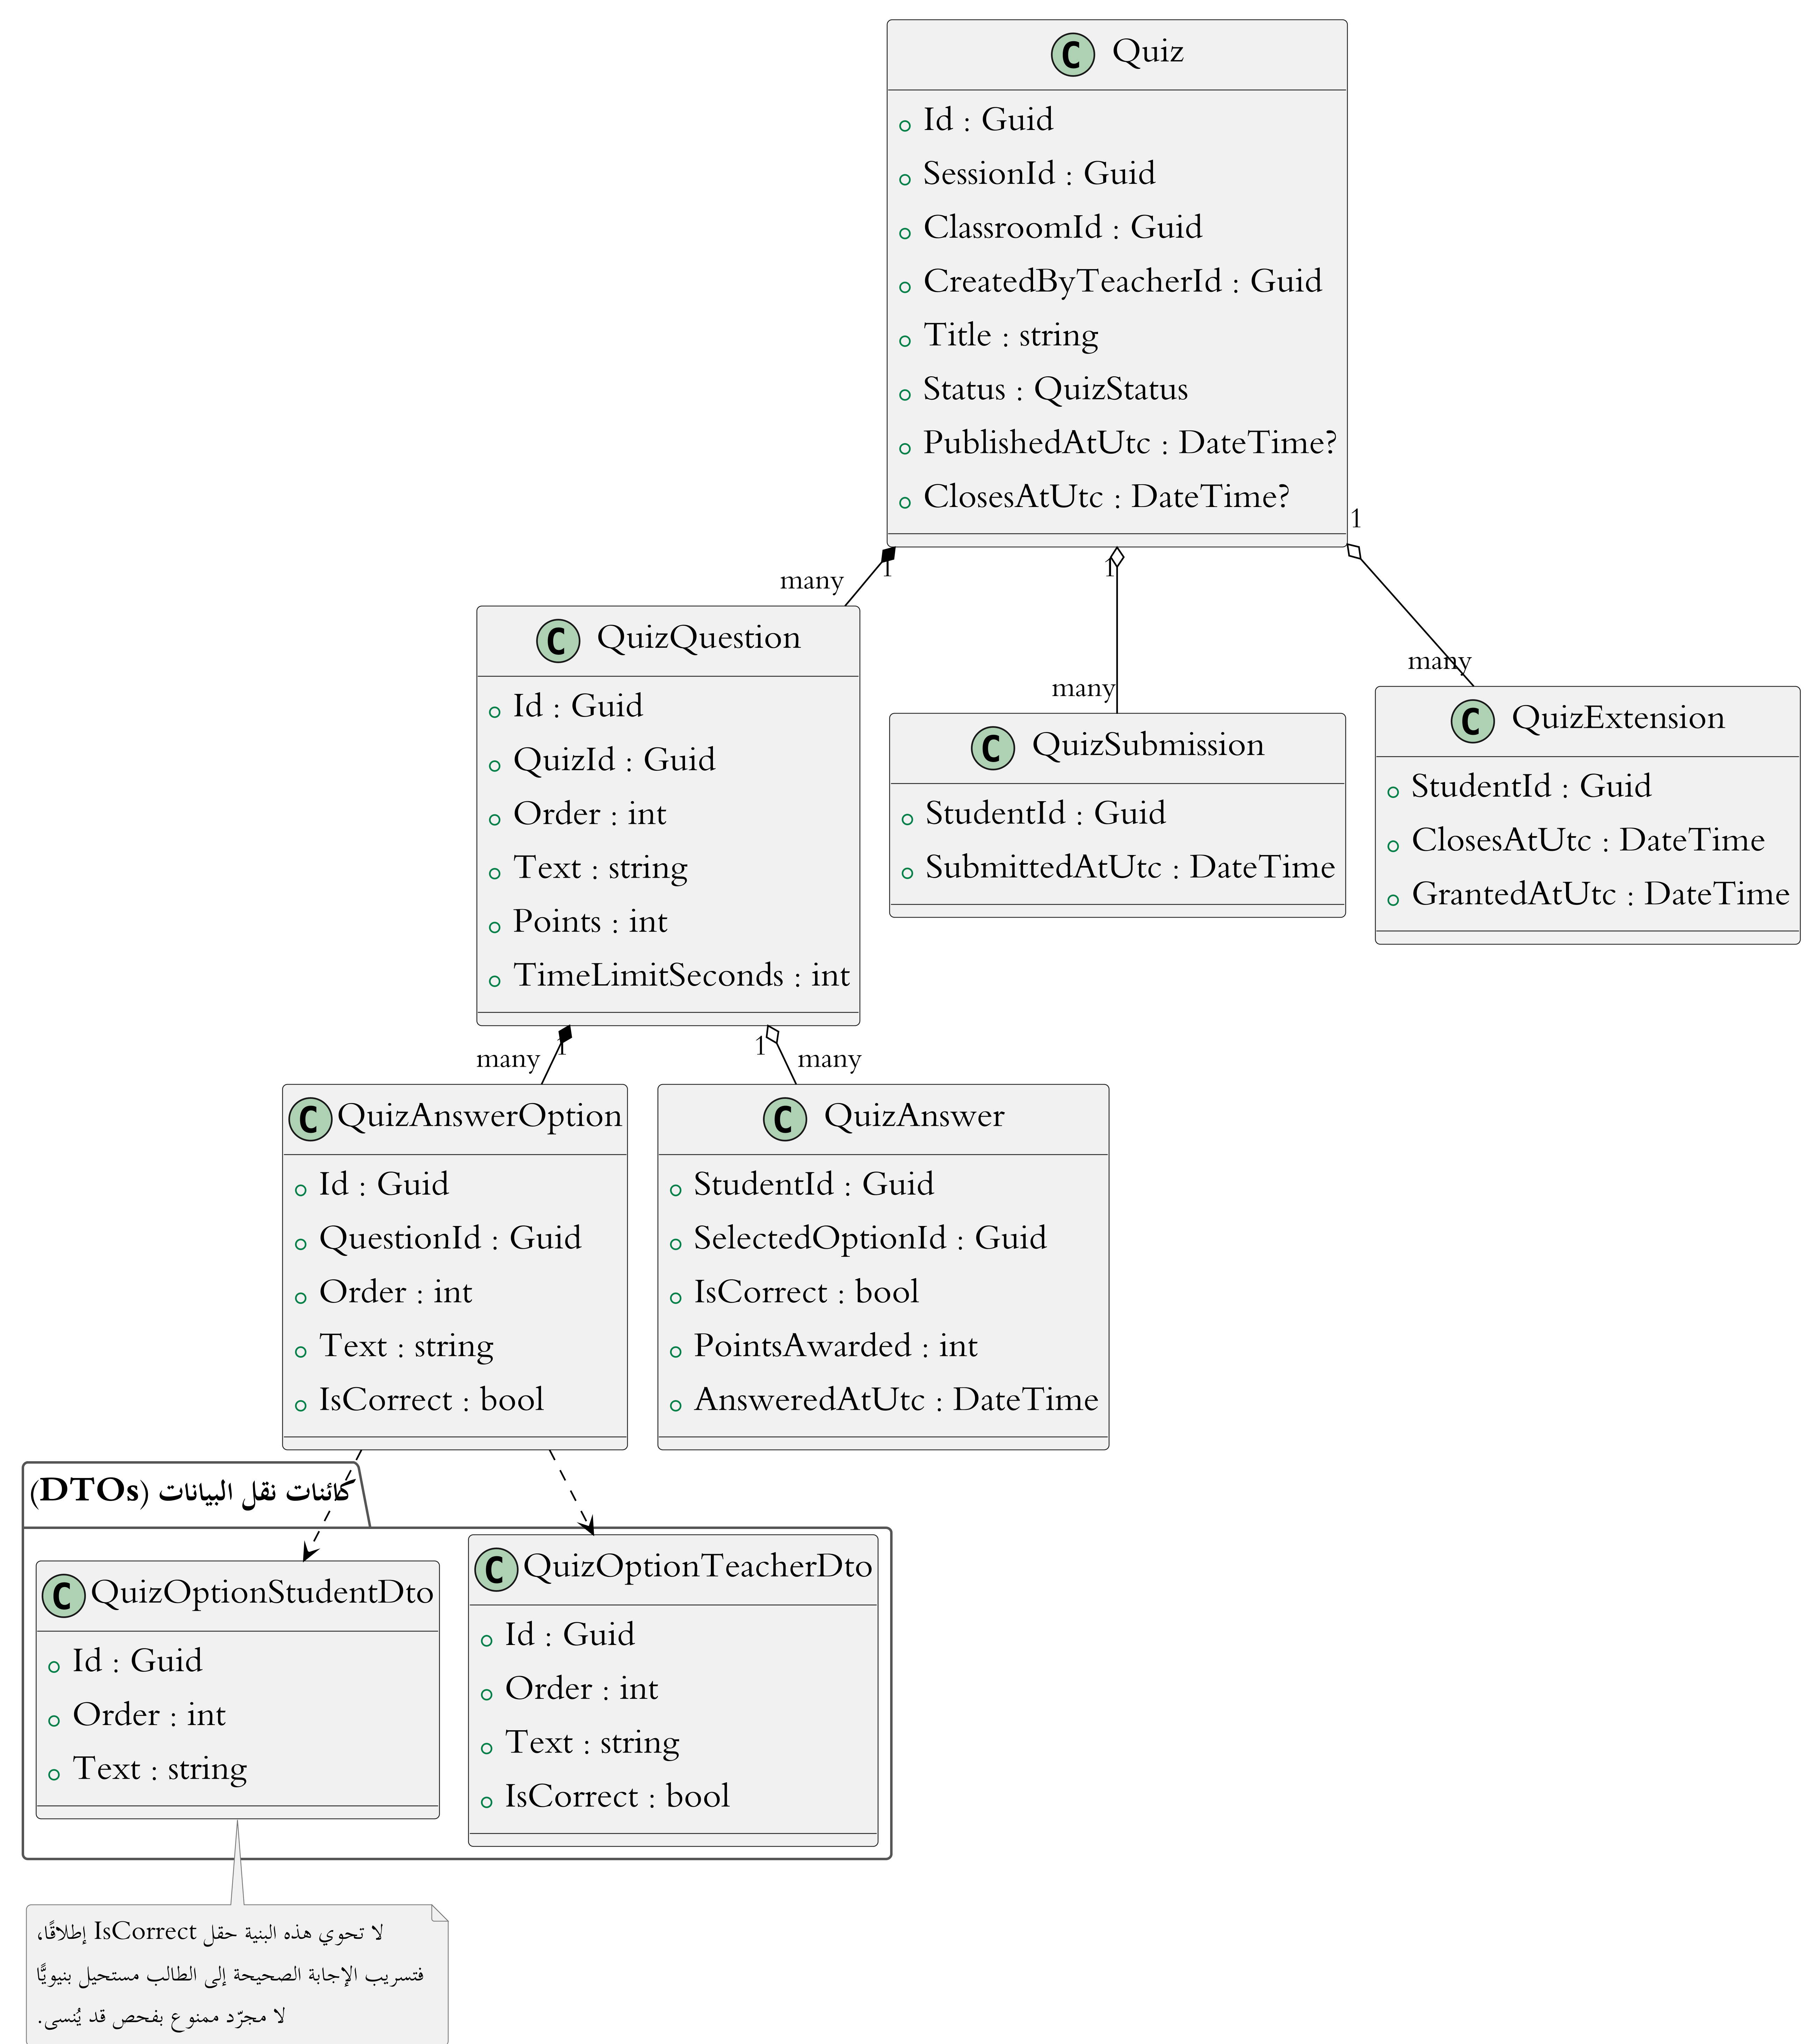
\includegraphics[width=\textwidth,height=0.8\textheight,keepaspectratio]{figures/class-02-quiz-domain.png}
  \caption{مخطط الصفوف لتجميعة الاختبار في خدمة الفصول الدراسية.}
  \label{fig:class-02}
\end{figure}

ويُحفظ الخيار الصحيح لكل سؤال في الحقل \en{IsCorrect} ضمن الكيان \en{QuizAnswerOption}. ولمنع وصول هذا الحقل إلى الطالب، عُرّفت بنيتان منفصلتان لنقل البيانات: بنية للمعلّم تتضمّن الحقل، وبنية للطالب لا تتضمّنه. ويمنع هذا الفصل البنيوي تسريب الإجابة الصحيحة، خلافًا للفحص البرمجي الذي قد يُغفَل عند إضافة مسار جديد.

ويُبيَّن تدفّق إنهاء الجلسة الحيّة، وما يعالجه من مشكلات السباق والذرّية والترتيب، في القسم~\ref{subsubsec:flow-session-end}.
